\documentclass[14pt]{extbook}
\usepackage{multicol, enumerate, enumitem, hyperref, color, soul, setspace, parskip, fancyhdr} %General Packages
\usepackage{amssymb, amsthm, amsmath, bbm, latexsym, units, mathtools} %Math Packages
\everymath{\displaystyle} %All math in Display Style
% Packages with additional options
\usepackage[headsep=0.5cm,headheight=12pt, left=1 in,right= 1 in,top= 1 in,bottom= 1 in]{geometry}
\usepackage[usenames,dvipsnames]{xcolor}
\usepackage{dashrule}  % Package to use the command below to create lines between items
\newcommand{\litem}[1]{\item#1\hspace*{-1cm}\rule{\textwidth}{0.4pt}}
\pagestyle{fancy}
\lhead{Progress Quiz 10}
\chead{}
\rhead{Version B}
\lfoot{6232-9639}
\cfoot{}
\rfoot{Fall 2020}
\begin{document}

\begin{enumerate}
\litem{
Determine the vertical asymptotes and holes in the rational function below.\[ f(x) = \frac{8x^{3} +22 x^{2} -21 x -45}{6x^{2} -x -12} \]\begin{enumerate}[label=\Alph*.]
\item \( \text{Vertical Asymptote of } x = 1.333 \text{ and hole at } x = 1.5 \)
\item \( \text{Vertical Asymptote of } x = -1.333 \text{ and hole at } x = 1.5 \)
\item \( \text{Vertical Asymptotes of } x = -1.333 \text{ and } x = -1.25 \text{ with a hole at } x = 1.5 \)
\item \( \text{Vertical Asymptotes of } x = -1.333 \text{ and } x = 1.5 \text{ with no holes.} \)
\item \( \text{Holes at } x = -1.333 \text{ and } x = 1.5 \text{ with no vertical asymptotes.} \)

\end{enumerate} }
\litem{
Determine the horizontal and/or oblique asymptotes in the rational function below.\[ f(x) = \frac{8x^{3} +14 x^{2} -35 x -50}{2x^{2} +9 x + 10} \]\begin{enumerate}[label=\Alph*.]
\item \( \text{Horizontal Asymptote of } y = -2.0 \text{ and Oblique Asymptote of } y = 4x -11 \)
\item \( \text{Horizontal Asymptote at } y = -2.0 \)
\item \( \text{Horizontal Asymptote of } y = 4.0 \text{ and Oblique Asymptote of } y = 4x -11 \)
\item \( \text{Horizontal Asymptote of } y = 4.0  \)
\item \( \text{Oblique Asymptote of } y = 4x -11. \)

\end{enumerate} }
\litem{
Which of the following functions \textit{could} be the graph below?
\begin{center}
    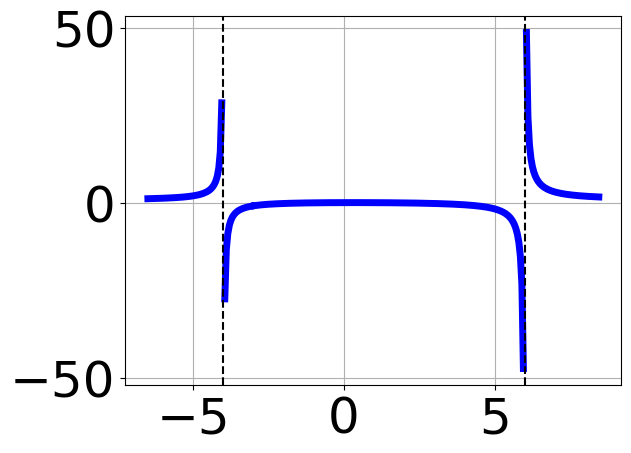
\includegraphics[width=0.5\textwidth]{../Figures/identifyGraphOfRationalFunctionB.png}
\end{center}
\begin{enumerate}[label=\Alph*.]
\item \( f(x)=\frac{x^{3} -2 x^{2} -9 x + 18}{x^{3} -1 x^{2} -30 x + 72} \)
\item \( f(x)=\frac{x^{3} + x^{2} -8 x -12}{x^{3} + x^{2} -30 x -72} \)
\item \( f(x)=\frac{x^{3} -2 x^{2} -9 x + 18}{x^{3} -1 x^{2} -30 x + 72} \)
\item \( f(x)=\frac{x^{3} +2 x^{2} -9 x -18}{x^{3} + x^{2} -30 x -72} \)
\item \( \text{None of the above are possible equations for the graph.} \)

\end{enumerate} }
\litem{
Determine the vertical asymptotes and holes in the rational function below.\[ f(x) = \frac{6x^{3} +43 x^{2} +86 x + 40}{6x^{2} +11 x -10} \]\begin{enumerate}[label=\Alph*.]
\item \( \text{Vertical Asymptotes of } x = 0.667 \text{ and } x = -2.5 \text{ with no holes.} \)
\item \( \text{Vertical Asymptote of } x = 1.0 \text{ and hole at } x = -2.5 \)
\item \( \text{Vertical Asymptotes of } x = 0.667 \text{ and } x = -0.667 \text{ with a hole at } x = -2.5 \)
\item \( \text{Vertical Asymptote of } x = 0.667 \text{ and hole at } x = -2.5 \)
\item \( \text{Holes at } x = 0.667 \text{ and } x = -2.5 \text{ with no vertical asymptotes.} \)

\end{enumerate} }
\litem{
Determine the horizontal and/or oblique asymptotes in the rational function below.\[ f(x) = \frac{12x^{3} +41 x^{2} -10 x -75}{15x^{3} +62 x^{2} +131 x + 60} \]\begin{enumerate}[label=\Alph*.]
\item \( \text{Vertical Asymptote of } y = -0.800  \)
\item \( \text{None of the above} \)
\item \( \text{Horizontal Asymptote of } y = 0.800  \)
\item \( \text{Horizontal Asymptote of } y = 0  \)
\item \( \text{Vertical Asymptote of } y = -3  \)

\end{enumerate} }
\litem{
Which of the following functions \textit{could} be the graph below?
\begin{center}
    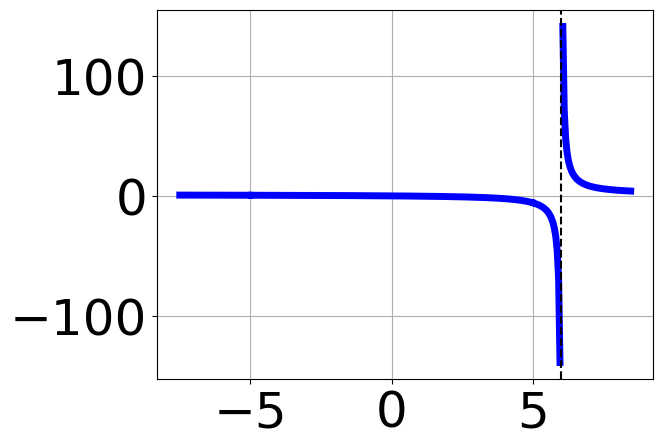
\includegraphics[width=0.5\textwidth]{../Figures/identifyGraphOfRationalFunctionCopyB.png}
\end{center}
\begin{enumerate}[label=\Alph*.]
\item \( f(x)=\frac{x^{3} -1 x^{2} -25 x + 25}{x^{3} +6 x^{2} -25 x -150} \)
\item \( f(x)=\frac{x^{3} + x^{2} -25 x -25}{x^{3} -6 x^{2} -25 x + 150} \)
\item \( f(x)=\frac{x^{3} -1 x^{2} -25 x + 25}{x^{3} +6 x^{2} -25 x -150} \)
\item \( f(x)=\frac{x^{3} +4 x^{2} -15 x -18}{x^{3} -6 x^{2} -25 x + 150} \)
\item \( \text{None of the above are possible equations for the graph.} \)

\end{enumerate} }
\litem{
Determine the horizontal and/or oblique asymptotes in the rational function below.\[ f(x) = \frac{6x^{3} -31 x^{2} +8 x + 80}{2x^{2} -x -10} \]\begin{enumerate}[label=\Alph*.]
\item \( \text{Horizontal Asymptote at } y = -2.0 \)
\item \( \text{Horizontal Asymptote of } y = 3.0  \)
\item \( \text{Horizontal Asymptote of } y = -2.0 \text{ and Oblique Asymptote of } y = 3x -14 \)
\item \( \text{Oblique Asymptote of } y = 3x -14. \)
\item \( \text{Horizontal Asymptote of } y = 3.0 \text{ and Oblique Asymptote of } y = 3x -14 \)

\end{enumerate} }
\litem{
Determine the vertical asymptotes and holes in the rational function below.\[ f(x) = \frac{6x^{3} +13 x^{2} -25 x -50}{9x^{2} +9 x -10} \]\begin{enumerate}[label=\Alph*.]
\item \( \text{Vertical Asymptotes of } x = 0.667 \text{ and } x = -2.5 \text{ with a hole at } x = -1.667 \)
\item \( \text{Holes at } x = 0.667 \text{ and } x = -1.667 \text{ with no vertical asymptotes.} \)
\item \( \text{Vertical Asymptote of } x = 0.667 \text{ and hole at } x = -1.667 \)
\item \( \text{Vertical Asymptotes of } x = 0.667 \text{ and } x = -1.667 \text{ with no holes.} \)
\item \( \text{Vertical Asymptote of } x = 0.667 \text{ and hole at } x = -1.667 \)

\end{enumerate} }
\litem{
Determine the horizontal and/or oblique asymptotes in the rational function below.\[ f(x) = \frac{18x^{3} -21 x^{2} -7 x + 10}{30x^{3} -68 x^{2} +58 x -15} \]\begin{enumerate}[label=\Alph*.]
\item \( \text{None of the above} \)
\item \( \text{Horizontal Asymptote of } y = 0  \)
\item \( \text{Vertical Asymptote of } y = 1  \)
\item \( \text{Vertical Asymptote of } y = 0.600  \)
\item \( \text{Horizontal Asymptote of } y = 0.600  \)

\end{enumerate} }
\litem{
Determine the vertical asymptotes and holes in the rational function below.\[ f(x) = \frac{6x^{3} -37 x^{2} +58 x -24}{8x^{2} -18 x + 9} \]\begin{enumerate}[label=\Alph*.]
\item \( \text{Vertical Asymptote of } x = 0.75 \text{ and hole at } x = 1.5 \)
\item \( \text{Vertical Asymptotes of } x = 0.75 \text{ and } x = 1.5 \text{ with no holes.} \)
\item \( \text{Holes at } x = 0.75 \text{ and } x = 1.5 \text{ with no vertical asymptotes.} \)
\item \( \text{Vertical Asymptotes of } x = 0.75 \text{ and } x = 0.667 \text{ with a hole at } x = 1.5 \)
\item \( \text{Vertical Asymptote of } x = 0.75 \text{ and hole at } x = 1.5 \)

\end{enumerate} }
\end{enumerate}

\end{document}